\chapter{Mock-up}
\label{s:mockup}


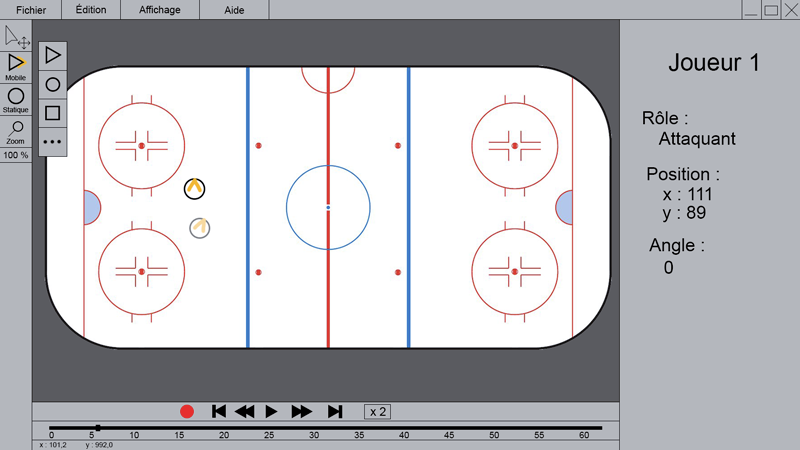
\includegraphics[scale=0.55]{mockup/mockup.png}

\section{Description}

\subsection{Section du centre}

Cette section est celle où la scène est affichée. Dans le fond de la scène s'affiche le terrain. C'est dans cette section où les éléments sont placés. En plaçant la sourie sur un élément, une icône s'affiche. En appuyant dessus, il est possible de modifier l'angle de l'élément.

\subsection{Section de droite}

Cette section contient les paramètres de l'élément actuellement sélectionné. Le premier champ, où il est écrit "Joueur 1", est le nom de l'élément. Le "Attaquant" est le rôle du joueur. C'est une comboBox dans laquelle les valeurs sont celles entrées dans les paramètres du sport. La position en x et en y de l'élément est modifiable via des champs numériques. L'angle aussi modifiable en utilisant un slider. Notez qu'il n'y a pas de rôle pour les éléments statiques et les balles.

\subsection{Section du bas}

Cette section permet de gérer la visualisation de la stratégie. Le cercle rouge permet de démarrer l'enregistrement de la stratégie. Les autres boutons sont les boutons traditionnels lors du visionnement de vidéo. Le x2 est dans un champ numérique. En changeant la valeur, on modifie la vitesse de défilement lors d'avance rapide et de recul. Notez que le "x" est seulement présent pour l'affichage. Lorsqu'on édite le champ, il n'est pas présent.


En dessous se trouve une ligne du temps. Le rectangle noir, le curseur, indique quelle image est affichée dans la scène. En le modifiant, l'image affichée dans la scène change. On peut voir juste en dessous la position en x et en y de la souris.

\subsection{Section de gauche}

Cette section contient les boutons permettant d'ajouter des éléments à la scène. C'est la barre d'outils. Le premier à partir du haut est celui utilisé pour déplacer les éléments. Le second sert à créer les éléments mobiles. Le troisième sert à créer les éléments statiques. En maintenant un clic sur le second et le troisième bouton, des icônes apparaissent à droite. Ils permettent de modifier l'élément qui sera ajouté à la scène grâce aux outils d'ajout d'éléments. Le quatrième bouton sert à zoomer sur la scène. Juste en dessous se trouve un champ numérique, permettant de modifier le zoom. 
